
\documentclass[border=10pt, 12pt]{standalone}
\usepackage[svgnames]{xcolor}
\usepackage{amsmath}
\usepackage{pgfplots}
\pgfplotsset{compat=newest}
\usepackage[sfdefault]{FiraSans}
\usepackage{FiraMono}
\renewcommand*\familydefault{\sfdefault}
\begin{document}
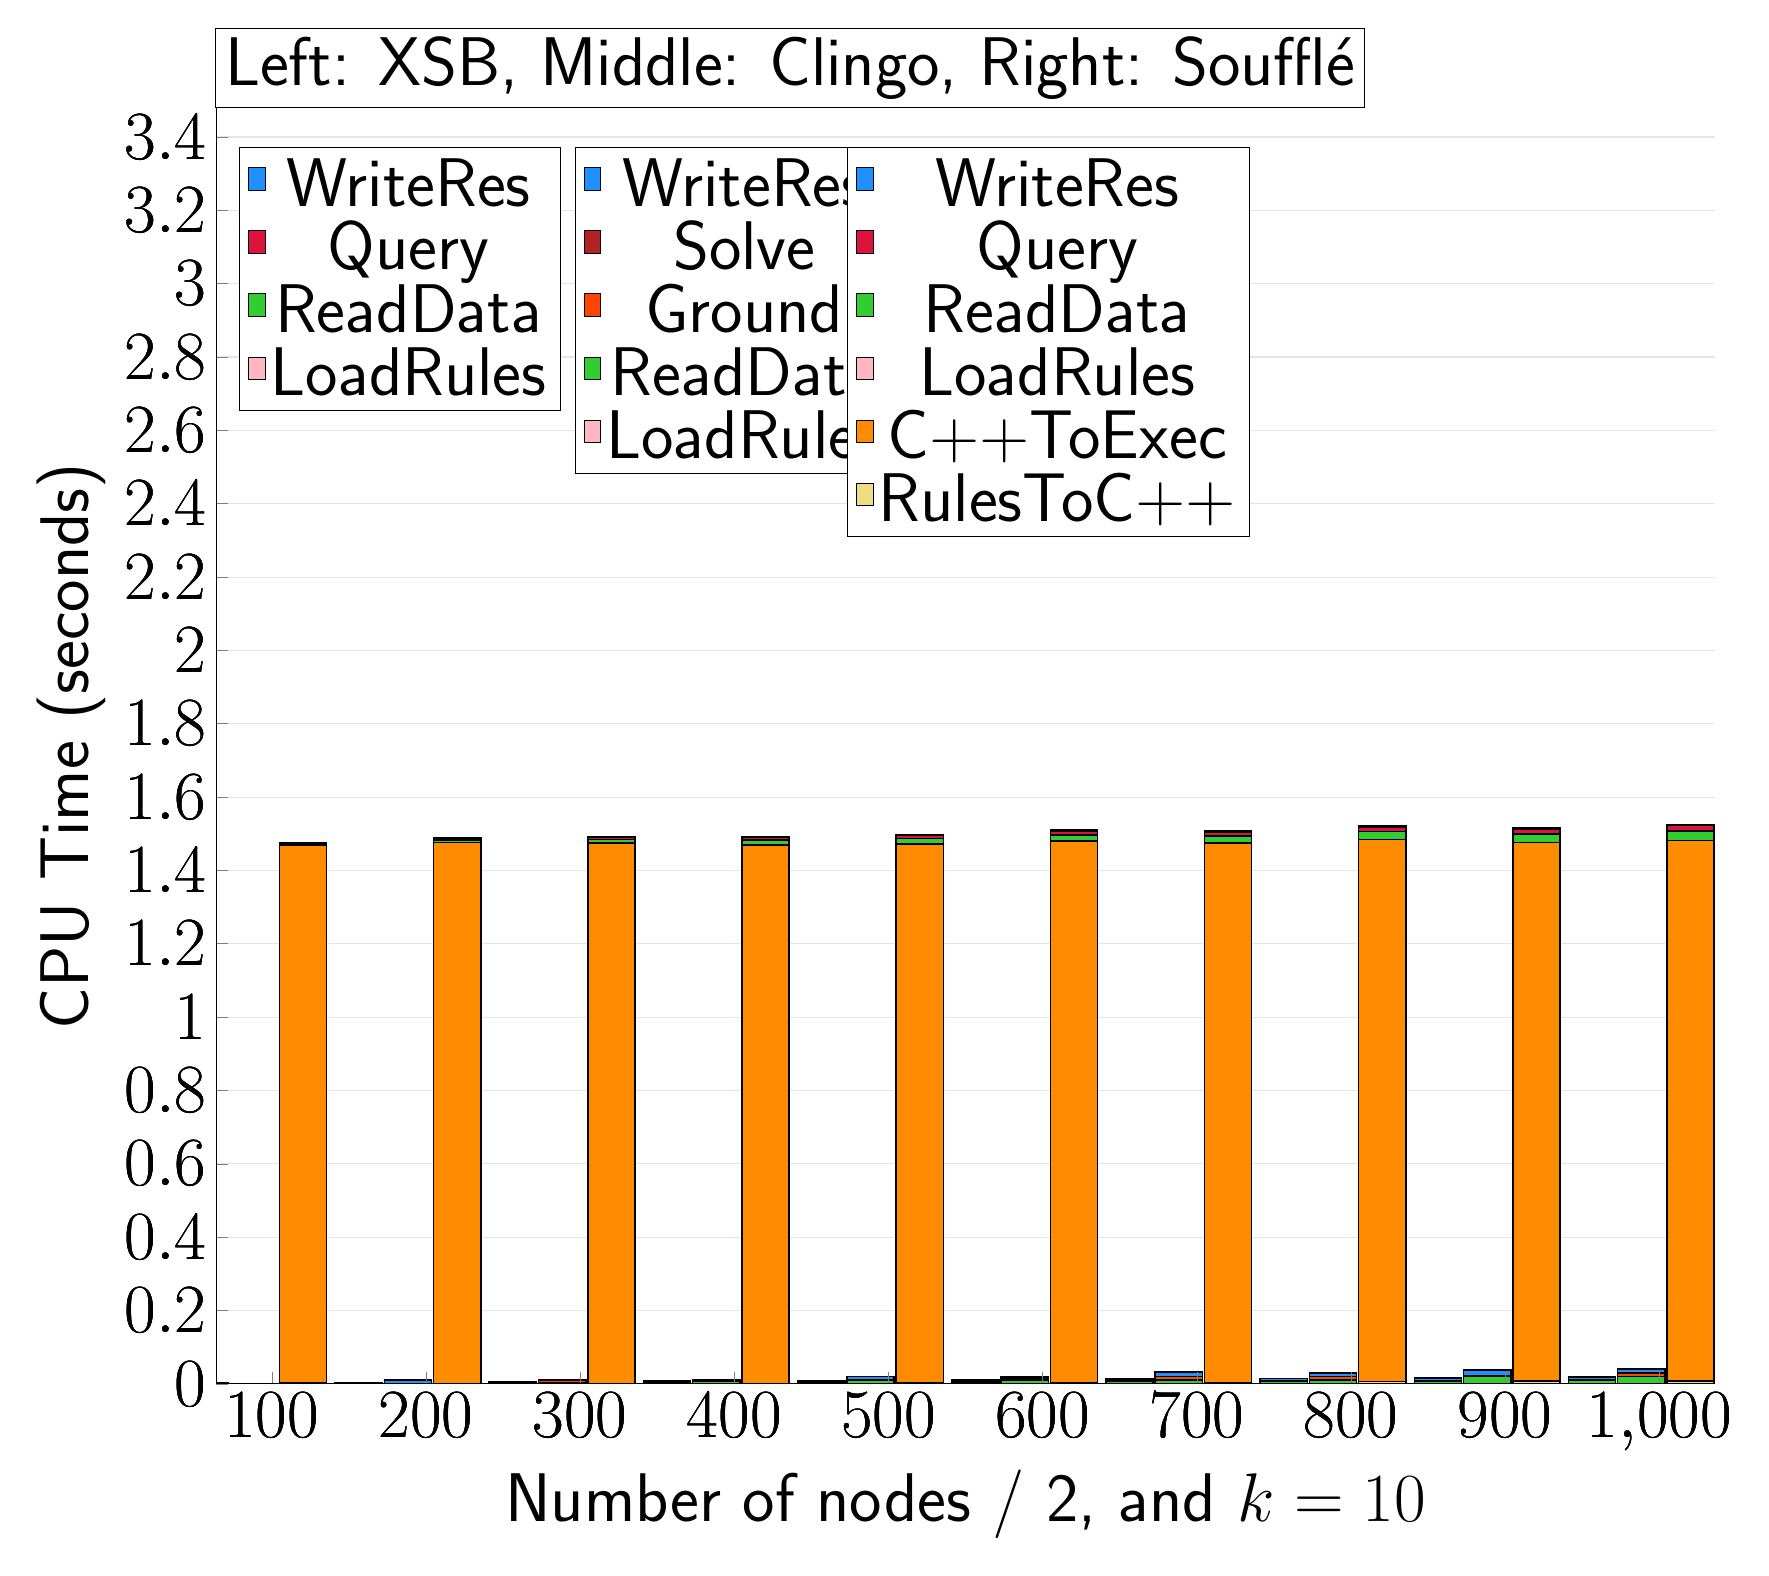
\begin{tikzpicture}
                        \begin{axis}[bar shift=-24.3pt, 
   ybar stacked,
   width=1.7\textwidth,
   bar width=0.6cm,
   ymajorgrids, tick align=inside,
   major grid style={draw=gray!20},
   xtick=data,
   ymin=0, ymax=3.4779999999999998,
   axis x line*=bottom,
   axis y line*=left,
   enlarge x limits=0.04,
   legend style={
       at={(0.23, 0.97)},
       anchor=north east,
       legend columns=1,
       font=\Huge,
   },
   ylabel={CPU Time (seconds)},
   xlabel={Number of nodes / 2, and $k=10$},
   label style={font=\Huge},
   tick label style={font=\Huge},
]
\addlegendimage{fill=DodgerBlue, draw=black, line width=0.2pt}
\addlegendentry{WriteRes}
\addlegendimage{fill=Crimson, draw=black, line width=0.2pt}
\addlegendentry{Query}
\addlegendimage{fill=LimeGreen, draw=black, line width=0.2pt}
\addlegendentry{ReadData}
\addlegendimage{fill=LightPink, draw=black, line width=0.2pt}
\addlegendentry{LoadRules}
\addplot +[fill=LightPink, draw=black, line width=0.55pt] coordinates {
(100, 0.0005510000000000005)
(200, 0.000554)
(300, 0.0005679999999999994)
(400, 0.0005510000000000003)
(500, 0.0005533999999999996)
(600, 0.0005514)
(700, 0.0005489999999999996)
(800, 0.0005649999999999996)
(900, 0.0005548000000000003)
(1000, 0.0005561999999999998)
};
\addplot +[fill=LimeGreen, draw=black, line width=0.55pt] coordinates {
(100, 0.0009004)
(200, 0.0016862)
(300, 0.0024952000000000004)
(400, 0.0032686)
(500, 0.004089799999999999)
(600, 0.004876799999999999)
(700, 0.0057428)
(800, 0.0066014)
(900, 0.007381)
(1000, 0.0082178)
};
\addplot +[fill=Crimson, draw=black, line width=0.55pt] coordinates {
(100, 0.0001297999999999996)
(200, 0.00024799999999999963)
(300, 0.00037899999999999924)
(400, 0.0005007999999999993)
(500, 0.0006274000000000003)
(600, 0.0007428000000000007)
(700, 0.0008536000000000001)
(800, 0.0009845999999999998)
(900, 0.0011194)
(1000, 0.0012406000000000001)
};
\addplot +[fill=DodgerBlue, draw=black, line width=0.55pt] coordinates {
(100, 0.0008742000000000005)
(200, 0.0016578000000000005)
(300, 0.002478000000000001)
(400, 0.003312800000000001)
(500, 0.004119)
(600, 0.004918199999999999)
(700, 0.0057748)
(800, 0.006548000000000001)
(900, 0.0073366)
(1000, 0.008137599999999998)
};
\end{axis}

\begin{axis}[bar shift=-6.5pt, 
   ybar stacked,
   width=1.7\textwidth,
   bar width=0.6cm,
   ymajorgrids, tick align=inside,
   major grid style={draw=none},
   xtick=data,
   ymin=0, ymax=3.4779999999999998,
   axis x line*=none,
   axis y line*=none,
   enlarge x limits=0.04,
   legend style={
       at={(0.454, 0.97)},
       anchor=north east,
       legend columns=1,
       font=\Huge,
   },
   label style={font=\Huge},
   tick label style={font=\Huge},
]
\addlegendimage{fill=DodgerBlue, draw=black, line width=0.2pt}
\addlegendentry{WriteRes}
\addlegendimage{fill=FireBrick, draw=black, line width=0.2pt}
\addlegendentry{Solve}
\addlegendimage{fill=OrangeRed, draw=black, line width=0.2pt}
\addlegendentry{Ground}
\addlegendimage{fill=LimeGreen, draw=black, line width=0.2pt}
\addlegendentry{ReadData}
\addlegendimage{fill=LightPink, draw=black, line width=0.2pt}
\addlegendentry{LoadRules}
\addplot +[fill=LightPink, draw=black, line width=0.55pt] coordinates {
(100, 0.0)
(200, 0.0)
(300, 0.0)
(400, 0.0)
(500, 0.0)
(600, 0.0)
(700, 0.0)
(800, 0.0)
(900, 0.0)
(1000, 0.0)
};
\addplot +[fill=LimeGreen, draw=black, line width=0.55pt] coordinates {
(100, 0.0)
(200, 0.0)
(300, 0.0020000000000000018)
(400, 0.008000000000000007)
(500, 0.010000000000000009)
(600, 0.010000000000000009)
(700, 0.010000000000000009)
(800, 0.010000000000000009)
(900, 0.020000000000000018)
(1000, 0.020000000000000018)
};
\addplot +[fill=OrangeRed, draw=black, line width=0.55pt] coordinates {
(100, 0.0)
(200, 0.0)
(300, 0.008000000000000007)
(400, 0.0020000000000000018)
(500, 0.0)
(600, 0.0040000000000000036)
(700, 0.010000000000000009)
(800, 0.010000000000000009)
(900, 0.0020000000000000018)
(1000, 0.010000000000000009)
};
\addplot +[fill=FireBrick, draw=black, line width=0.55pt] coordinates {
(100, 0.0)
(200, 0.0)
(300, 0.0)
(400, 0.0)
(500, 0.0)
(600, 0.0040000000000000036)
(700, 0.0)
(800, 0.0)
(900, 0.0)
(1000, 0.0)
};
\addplot +[fill=DodgerBlue, draw=black, line width=0.55pt] coordinates {
(100, 0.0)
(200, 0.010000000000000009)
(300, 0.0)
(400, 0.0)
(500, 0.010000000000000009)
(600, -0.0020000000000000018)
(700, 0.012000000000000009)
(800, 0.010000000000000009)
(900, 0.016000000000000014)
(1000, 0.010000000000000009)
};
\end{axis}

\begin{axis}[bar shift=11.3pt, 
   ybar stacked,
   width=1.7\textwidth,
   bar width=0.6cm,
   ymajorgrids, tick align=inside,
   major grid style={draw=none},
   xtick=data,
   ymin=0, ymax=3.4779999999999998,
   axis x line*=none,
   axis y line*=none,
   enlarge x limits=0.04,
   legend style={
       at={(0.69, 0.97)},
       anchor=north east,
       legend columns=1,
       font=\Huge,
   },
   label style={font=\Huge},
   tick label style={font=\Huge},
]
\addlegendimage{fill=DodgerBlue, draw=black, line width=0.2pt}
\addlegendentry{WriteRes}
\addlegendimage{fill=Crimson, draw=black, line width=0.2pt}
\addlegendentry{Query}
\addlegendimage{fill=LimeGreen, draw=black, line width=0.2pt}
\addlegendentry{ReadData}
\addlegendimage{fill=LightPink, draw=black, line width=0.2pt}
\addlegendentry{LoadRules}
\addlegendimage{fill=DarkOrange, draw=black, line width=0.2pt}
\addlegendentry{C++ToExec}
\addlegendimage{fill=LightGoldenrod, draw=black, line width=0.2pt}
\addlegendentry{RulesToC++}
\addplot +[fill=LightGoldenrod, draw=black, line width=0.55pt] coordinates {
(100, 0.0020000000000000005)
(200, 0.0)
(300, 0.0)
(400, 0.0)
(500, 0.0020000000000000005)
(600, 0.0020000000000000005)
(700, 0.004000000000000001)
(800, 0.006000000000000001)
(900, 0.008000000000000002)
(1000, 0.008000000000000002)
};
\addplot +[fill=DarkOrange, draw=black, line width=0.55pt] coordinates {
(100, 1.466)
(200, 1.4760000000000002)
(300, 1.474)
(400, 1.47)
(500, 1.47)
(600, 1.478)
(700, 1.47)
(800, 1.478)
(900, 1.4679999999999997)
(1000, 1.4739999999999998)
};
\addplot +[fill=LightPink, draw=black, line width=0.55pt] coordinates {
(100, 0.0001878)
(200, 0.0001974)
(300, 0.000203)
(400, 0.00018180000000000003)
(500, 0.0001872)
(600, 0.0001932)
(700, 0.00020940000000000005)
(800, 0.0002032)
(900, 0.00019020000000000002)
(1000, 0.00019080000000000003)
};
\addplot +[fill=LimeGreen, draw=black, line width=0.55pt] coordinates {
(100, 0.0037862)
(200, 0.006628)
(300, 0.009843000000000001)
(400, 0.0124748)
(500, 0.014846600000000001)
(600, 0.0171172)
(700, 0.0190068)
(800, 0.021344000000000002)
(900, 0.0237288)
(1000, 0.025286399999999997)
};
\addplot +[fill=Crimson, draw=black, line width=0.55pt] coordinates {
(100, 0.0022955999999999996)
(200, 0.004228399999999999)
(300, 0.005621800000000001)
(400, 0.007285)
(500, 0.009364800000000001)
(600, 0.0102622)
(700, 0.0122452)
(800, 0.0130742)
(900, 0.0132492)
(1000, 0.0149468)
};
\addplot +[fill=DodgerBlue, draw=black, line width=0.55pt] coordinates {
(100, 0.0008972000000000001)
(200, 0.0013056)
(300, 0.0015212)
(400, 0.0020502)
(500, 0.0021754)
(600, 0.0024701999999999997)
(700, 0.0026672)
(800, 0.002826)
(900, 0.0031127999999999998)
(1000, 0.003223)
};
\end{axis}


\node[anchor=south, draw, fill=white] at (rel axis cs:0.42, 1) {\Huge Left: XSB, Middle: Clingo, Right: Soufflé};
\end{tikzpicture}
\end{document}
                    